\subsection{Постановка задачи}
1.3. Реализовать метод простых итераций и метод Зейделя в виде программ, задавая в качестве входных данных матрицу системы, вектор правых частей и точность вычислений. Используя разработанное программное обеспечение, решить СЛАУ. Проанализировать количество итераций, необходимое для достижения заданной точности.

{\bfseries Вариант:} 20
\begin{equation}
        \left\{ 
        \begin{array}{ll} 
        10x_1 - x_2 - 2x_3 + 5x_4 = -99 \\
        4x_1 + 28x_2 + 7x_3 + 9x_4 = 0\\
        6x_1 + 5x_2 - 23x_3 + 4x_4 = 67\\
        x_1 + 4x_2 + 5x_3 - 15x_4 = 58\\
        \end{array}\right.
\end{equation}
\pagebreak

\subsection{Результаты работы}

\begin{figure}[h!]
\centering
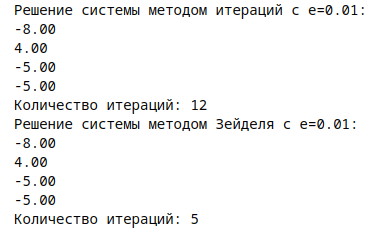
\includegraphics[width=.5\textwidth]{lab1.3}
\caption{Вывод в консоли}
\end{figure}
\pagebreak

\vfill

\subsection{Исходный код}

\lstinputlisting[title=\texttt{3.cpp}]{../stud/svoevolin/exercise_3/3.cpp}
\pagebreak